\chapter{Reference model\label{sec:reference_model}}
\par{
    As a reference to compare the models trained on weakly-supervised data with, the model performance of a model trained on the same fully supervised data is taken as a reference.
    In this chapter, the results of these fully supervised reference experiments are discussed.
    The metric based on which the experiment results are compared is the weighted dice score, see equation \ref{eq:weighted_dice} on page \pageref{eq:weighted_dice}.
}

\section{Experiment results}
\par{
    The fully supervised experiments serve two goals.
    First is to calculate a reference model performance with which to compare the weakly supervised model results.
    The second is to support hyperparameter choices for the point supervised experiments.
    It is assumed that a network architecture that yields a good fully supervised model is also a suitable choice to build a weakly supervised model.
    The possible influence of the context slices\footnote{The context slice idea is discussed in detail in chapter \ref{section:twoDplus} on page \pageref{section:twoDplus}.} is also evaluated with these experiments.
}
\par{
    In figure \ref{fig:referenceExperiments}, the results of the reference experiments are shown.
    These results show the network based on VGG16 yields better results than the alternatives based on RESNET50 and U-Net.
    Despite what was hoped for, the context slices do not seem to strongly increase the model performance.
    Remarkably, there is little difference between the models trained with a weighted cross-entropy loss and the non-weighted cross-entropy loss\footnote{
        The weighted cross entropy loss is defined in chapter \ref{sec:crossentropy} on page \pageref{sec:crossentropy}. 
        The objective of a weighted cross entropy is to improve the model performance for under-represented classes in an unbalanced dataset by adding a factor inverse proportional to the class prevalence to the cross entropy loss.
    } when considering the weighted dice score.
    In figures \ref{fig:referenceWeighted} and \ref{fig:referencenonWeighted}, the model result based on the FCN8 VGG16 model with context slices at 1 mm from the central slice is compared in detail for the models trained with weighted and the unweighted cross entropy function.
    Based on these images, some conclusions can be drawn:
    \begin{enumerate}
        \item The prediction of the background class is practically perfect, for all datasets.
        \item The model trained with an unweighted cross entropy loss underperforms compared to the model trained with the weighted cross entropy loss for the prediction of the $L1$ class.
    \end{enumerate}
}
\begin{SCfigure}[][htb]
    \centering
    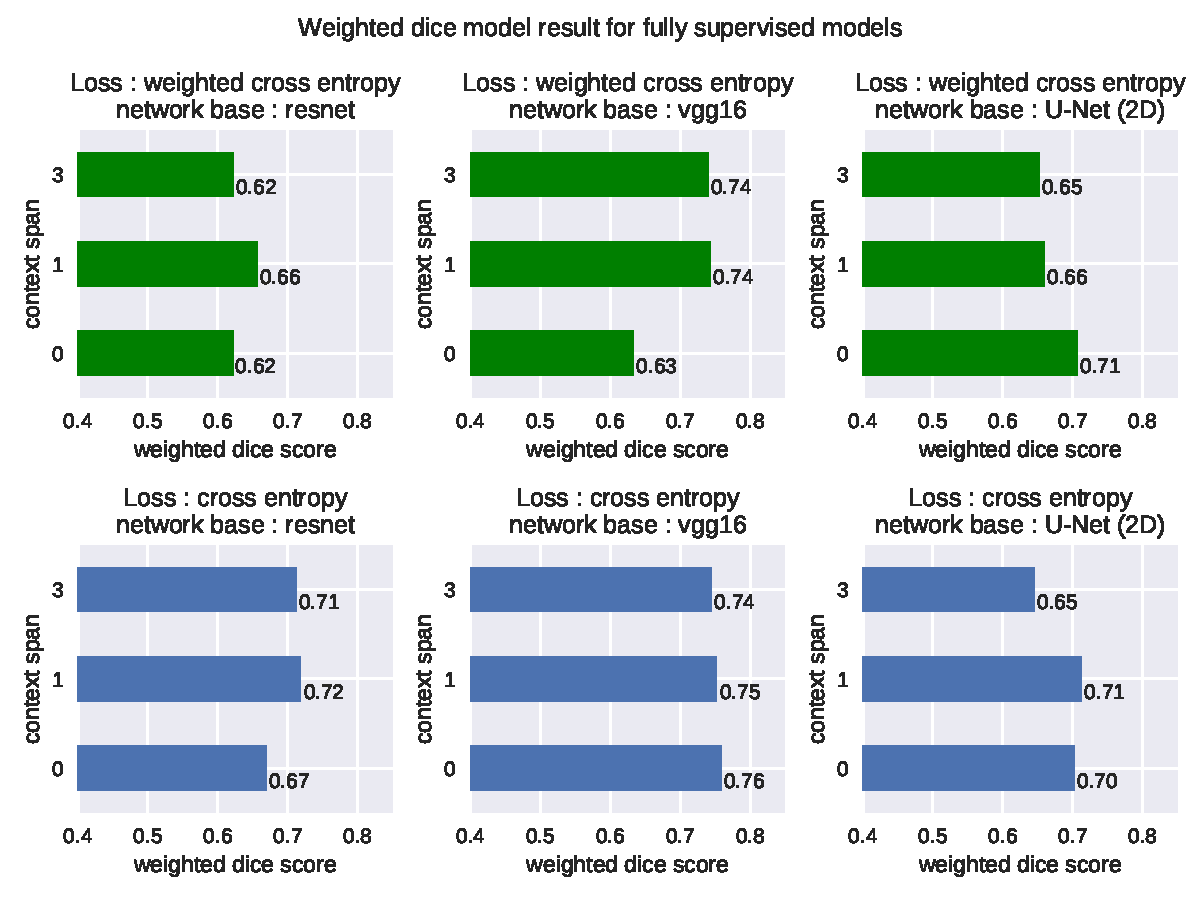
\includegraphics[width=.95\textwidth]{images/FullySupervised.pdf}
    \caption{Results of the fully supervised experiments.
    The indicated model performance metrics are calculated on the test set.
    The columns represent de weighted dice scores for models based on the same network architecture with different loss functions.
    \label{fig:referenceExperiments}}
\end{SCfigure}
\begin{SCfigure}[][htb]
    \centering
    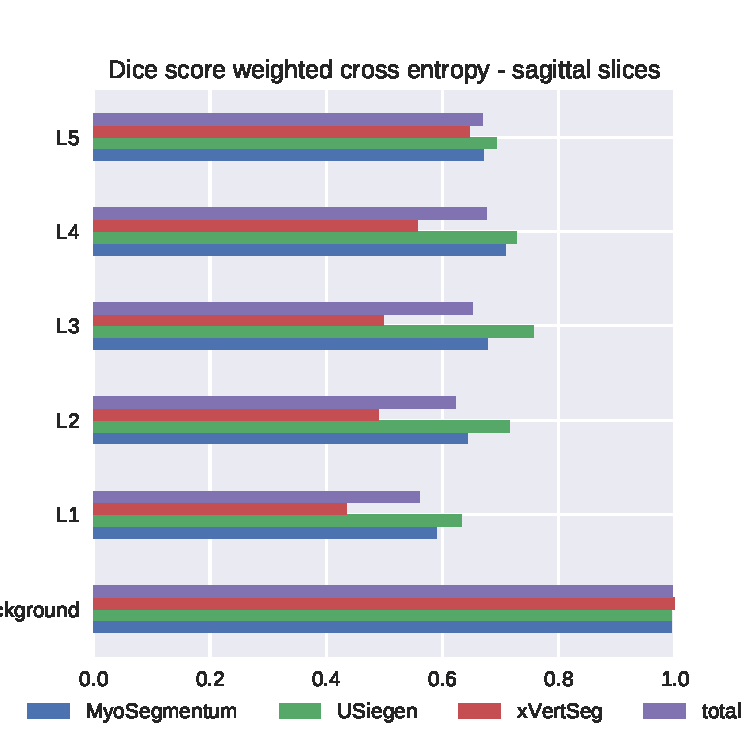
\includegraphics[width=.95\textwidth]{images/full_perClass_perSource_weighted.pdf}
    \caption{Detailed result for the fully supervised model trained with context slices at 1 mm from the central slice and with a weighted cross entropy loss function.
    \label{fig:referenceWeighted}}
\end{SCfigure}
\begin{SCfigure}[][htb]
    \centering
    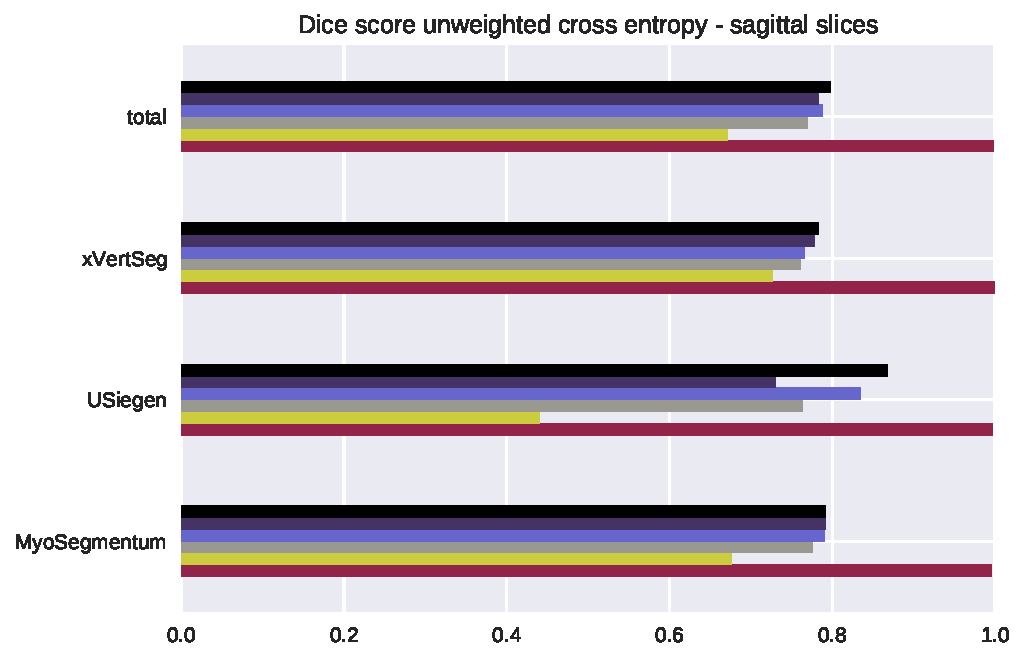
\includegraphics[width=.95\textwidth]{images/full_perClass_perSource_notweighted.pdf}
    \caption{Detailed result for the fully supervised model trained with context slices at 1 mm from the central slice and with a unweighted cross entropy loss function.
    \label{fig:referencenonWeighted}}
\end{SCfigure}



\section{Conclusion}
\par{
    Based on the results shown in figure \ref{fig:referenceExperiments}, it was decided to perform the weakly supervised experiments with the model based on VGG16 FCN8 with 1 context slice.
    The reference performance metric to compare experiments with models trained on weakly supervised data with is $\text{Dice}_w=0,76$.
}
